\documentclass{article}

\usepackage{amsmath}
\usepackage{graphicx}
\usepackage{xcolor}
\usepackage{listings}
\usepackage{amsfonts}
\usepackage{amssymb}
\usepackage{graphicx}
\usepackage{titling}
\usepackage[utf8]{inputenc}
\usepackage[english]{babel}
\usepackage{amsmath}
\usepackage{fancyhdr}
\usepackage{lastpage}
\usepackage{textcomp}
\usepackage{graphicx}
\usepackage{hyperref}
\usepackage{float}

\addtolength{\oddsidemargin}{-.875in}
\addtolength{\evensidemargin}{-.875in}
\addtolength{\textwidth}{1.75in}
\addtolength{\topmargin}{-.875in}
\addtolength{\textheight}{1.75in}

\title{\Huge Applicazione Meteo \vspace{1cm}}
\author{Riccardo Biella, Nicol Allegra, Luca Ambrosio}
\date{Semestre primaverile 2019}
\setcounter{page}{0}
\pagestyle{fancy}
\fancyhf{}

\fancyfoot[C]{Page \thepage \hspace{1pt} of \pageref{LastPage}}

\begin{document}
\maketitle
\thispagestyle{empty}
\pagebreak


\tableofcontents
\lstset{language=C++}
\pagebreak

\section{Analisi del codice fornito}
Le applicazioni android vengono strutturate attraverso il pattern MVC, dove abbiamo i model, i layout e le activities/fragments, che si identificano rispettivamente in modelli, view e controller.
Prima di addentrarci nell'analisi del codice d'esempio fornito, dobbiamo introdurre il concetto di fragments: i fragments costituiscono una sorta di controller minori a cui le activities si appoggiano per l'esecuzione di alcuni task.
I fragments sono spesso utilizzati per gestire gli aggiornamenti della UI, in questo caso prendono il nome di UI fragments.
Per utilizzare i fragments è necessario che un'activity definisca un layout che dovra contenere i vari fragments.

\begin{figure}[H]
    \center
    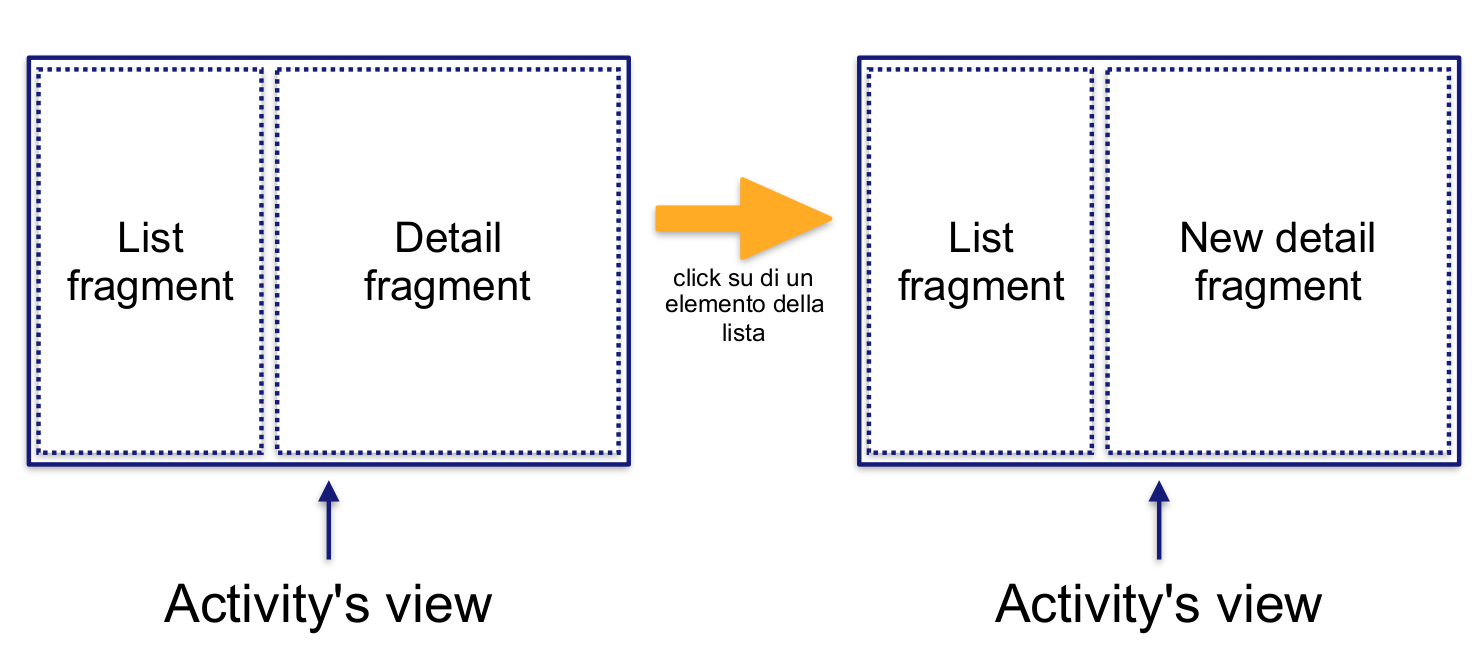
\includegraphics[scale=0.25]{images/fig1.png}
\end{figure}

\subsection{Package activities}
\begin{itemize} 
    \item \textbf{SingleFragmentActivity} \\
    Nel caso più semplice, una view di un’attività contiene semplicemente un fragment. In questo caso il modo più elegante di procedere
    consiste nel dichiare un'activity astratta che andrà estesa dalle activities che sono gestite da un singolo frammento.
    In questa classe astratta si rimanda alle sottoclassi che la estenderanno, l'implementazione del metodo createFragment(), che deve essere
    differente per ogni classe figlia, mentre si implementa il metodo onCreate():
    \begin{lstlisting}
    @Override
    protected void onCreate(Bundle savedInstanceState) {
        super.onCreate(savedInstanceState);

        // Setto il layout "container" che conterrà i vari fragments
        setContentView(R.layout.fragment_single_fragment);

        // Instanzio un gestore di fragments
        FragmentManager fm = getSupportFragmentManager();

        // Tramite l'id che ho settato nel fragment_single_fragment.xml 
        // ottengo il mio fragment, controllo se è già istanziato
        // quando giro il telefono l'activity si distrugge ma i fragments no
        // vengono mantenuti dal gestore di fragments
        Fragment fragment = fm.findFragmentById(R.id.fragment_container);
        if (fragment == null) {
            fragment = createFragment();
            // applichiamo il cambiamento tramite le transactions
            fm.beginTransaction()
                    .add(R.id.fragment_container, fragment)
                    .commit();
        }
    }
    \end{lstlisting}
    Un'activity per essere tale deve estendere AppCompatActivity che permette di overraidare alcuni metodi utili.
    Il metodo onCreate() riceve come parametro un Bundle, un oggetto in cui è possibile salvare dei dati serializzati, questo è utile nel caso in cui giro il dispositivo
    e android distrugge e ricrea l'applicazione per passare da portrait a landscape, tramite questo oggetto posso salvare lo stato.
    \item \textbf{MainActivity} \\
    E' l'activity principale, è quella che viene lanciata all'avvio dell'applicazione. Tutte le activities sono indicate nell' AndroidManifest.xml
    automaticamente al momento della creazione, dall'editor; in questo file l'activity principale è indicata come LAUNCHER.
    Questa classe non fa altro che estendere la classe SingleFragmentActivity ed implementare il metodo astratto
    createFragment(), all'interno del quale viene instanziato un fragment a cui viene delegata l'intera gestione dell'attività.
    \item \textbf{DetailsActivity} \\
    Questa classe gestisce la visualizzazione della pagina di dettaglio, al momento del click dell'utente su una Location presente del menù.
    Anch'essa istanzia un fragment a cui delega la gestione della logica di business, ma a differenza della MainActivity implementa uno scambio di informazioni tra classi, tramite 
    l'utilizzo degli Intent Extra. Viene definito un factory metod chiamato newInstance() (Best practices) che può essere invocato dalle classi che hanno la necessità di 
    creare una DetailsActivity, in questo modo è la classe stessa a definire come vuole essere invocata, nel nostro caso necessita di un id per essere costistente.
    \begin{lstlisting}
public class DetailActivity extends SingleFragmentActivity {
private static final String EXTRA_LOCATION_ID = 
                    "ch.supsi.dti.isin.meteoapp.location_id";

public static Intent newIntent(Context packageContext, UUID locationId) {
    Intent intent = new Intent(packageContext, DetailActivity.class);
    // Inserisco nell'Intent, che funziona come una sorta di mappa, l'id che mi è
    // stato fornito dalla classe chiamante, con la chiave statica che definisco.
    intent.putExtra(EXTRA_LOCATION_ID, locationId);
    return intent;
}

// quando verrà invocato dalla classe chiamante: startActivity(intent), finiamo
// nel metodo onCreate() della classe astratta SingleFragmentActivity che esegue
// una chiamata al metodo seguente, dove recupero l'intent e l'informazione
// relativa alla location_id, attraverso la chiave con cui l'ho salvato.
@Override
protected Fragment createFragment() {
    UUID locationId = (UUID) getIntent().getSerializableExtra(EXTRA_LOCATION_ID);
    return new DetailLocationFragment().newInstance(locationId);
}
}
    \end{lstlisting}
\end{itemize}

\subsection{Package fragments}
\begin{itemize} 
    \item \textbf{DetailLocationFragment} \\
    Questa classe rappresenta il fragment invocato dall'activity che si occupa di gestire la visualizzazione del dettaglio
    di ogni location. Questo fragment definisce, analogamente a quanto visto per le activity, il modo in cui vuole essere invocato.
    Nel nostro caso il fragment necessita di un location\_id per essere costistente. Per passare argomenti ad un fragment si utilizza
    un meccanismo molto simile agli Intent Extra visti per le activity: ogni istanza di un fragment può contenere un oggetto di tipo Bundle. Il Bundle contiene delle coppie
    di chiave-valore che funzionano esattamente come gli extras di un’Activity. Per creare degli argomenti da
    passare ad un fragment, si crea prima l’oggetto Bundle, e poi si aggiungono i valori voluti.
    Nel metodo onCreate() troviamo invece la lettura del parametro passato attraverso il Bundle, e la ricerca all'interno della lista di località
    gestita dal LocationsHolder, dell'item corrispondente all'id della location che vogliamo gestire, di cui salviamo la referenza.  
    Nel metodo onCreateView() vengono salvate le referenze ai widgets interessati, nel nostro caso salviamo la referenza ad un textView.
    \item \textbf{ListFragment} \\
    Questa classe è sicuramente la più complessa della soluzione, dispone di due attributi, un RecyclerView e un Adapter.
    RecyclerView è un classe in grado di visualizzare una lista di figli di tipo View, i quali possono essere molto semplici o complessi.
    Questa classe gestisce le view in memoria, ad esempio se un utente scrolla la lista, la classe riusa le View che ha in memoria per visualizzare il nuovo contenuto,
    riciclandole continuamente.
    L’unica responsabilità del RecyclerView è quella di riciclare le Views e di posizionarle sullo schermo. Per 
    ”ottenere” le View, il RecyclerView necessita di due classi che vanno implementate: un Adapter e un ViewHolder.
    Il lavoro del ViewHolder è quello di ”tenere” una view. L’Adapter è invece responsabile
    di creare i ViewHolders necessari e di fare il bind dei ViewHolders ai dati (che sono contenuti nel Model).
    Un RecyclerView non crea mai le Views da solo, ma chiede ad un adapter di creare dei ViewHolders, i quali
    contengono le View.
    \begin{figure}[H]
        \center
        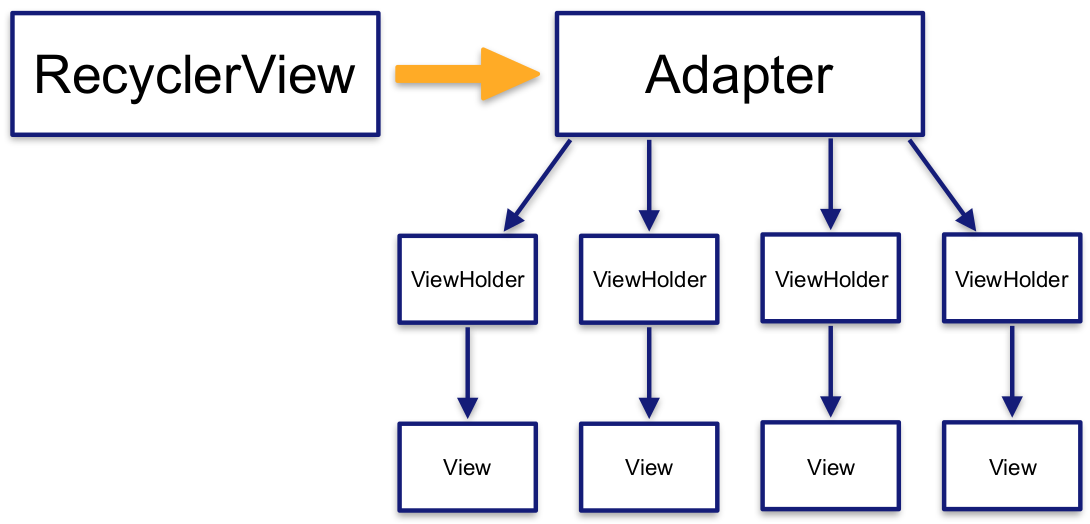
\includegraphics[scale=0.28]{images/fig2.png}
    \end{figure}
    Contestualizziamo ora i concetti espressi nel caso della nostra applicazione meteo.
    \begin{lstlisting}
// ViewHolder
private class LocationHolder extends RecyclerView.ViewHolder
                                 implements View.OnClickListener {
    private TextView mNameTextView;
    private Location mLocation;

    // viene definito il layout di ogni singola riga: list_item
    // l'istanza in questione viene settata come ascoltatore della
    // sua item, viene "recuperata" la referenza del widget sulla UI
    public LocationHolder(LayoutInflater inflater, ViewGroup parent) {
        super(inflater.inflate(R.layout.list_item, parent, false));
        itemView.setOnClickListener(this);
        mNameTextView = itemView.ViewById(R.id.name);
    }

    // sull'evento di click viene visualizzato il dettaglio della location
    @Override
    public void onClick(View view) {
        Intent intent = DetailActivity.newIntent(getActivity(), mLocation.getId());
        startActivity(intent);
    }

    // l'adapter utilizzerà questo metodo per fare il bind dei ViewHolder
    // con i dati che sono contenuti nel model
    public void bind(Location location) {
        mLocation = location;
        mNameTextView.setText(mLocation.getName());
    }
}
    \end{lstlisting}
\begin{lstlisting}
    // Adapter
    private class LocationAdapter extends RecyclerView.Adapter<LocationHolder> {
        private List<Location> mLocations;

        public LocationAdapter(List<Location> locations) {
            mLocations = locations;
        }

        // l'Adapter si occupa della creazione dei ViewHolders
        @Override
        public LocationHolder onCreateViewHolder(ViewGroup parent, int viewType) {
            LayoutInflater layoutInflater = LayoutInflater.from(getActivity());
            return new LocationHolder(layoutInflater, parent);
        }

        // l'Adapter si occupa di bindare i dati ai ViewHolders
        public void onBindViewHolder(LocationHolder holder, int position) {
            Location location = mLocations.get(position);
            holder.bind(location);
        }

        @Override
        public int getItemCount() {
            return mLocations.size();
        }
    }
\end{lstlisting}
In questa classe è stata utilizzata una toolbar ed un menù, questi ultimi sono gestiti dall’activity tramite callbacks. Quando è
necessario visualizzare un menu, Android chiama il metodo onCreateOptionsMenu(Menu). Il menu va prima
creato in un suo file XML. Si crea un XML che descrive il menu e lo si inserisce nella cartella res/menu. 
Il menu viene creato in Android Studio tramite tasto destro sulla cartella res e selezionando poi New –>
Android Resource File. Di norma ha lo stesso nome del fragment che lo ”contiene”. Nel nostro esempio troviamo il file
XML del menù all'interno della cartella res -> menu.
\begin{lstlisting}
    // In questo metodo viene iniettato il layout del menu.
    @Override
    public void onCreateOptionsMenu(Menu menu, MenuInflater inflater) {
        super.onCreateOptionsMenu(menu, inflater);
        inflater.inflate(R.menu.fragment_list, menu);
    }

    // in questo metodo si definiscono le azioni da compiere quando un'item
    // viene selezionata
    @Override
    public boolean onOptionsItemSelected(MenuItem item) {
        switch (item.getItemId()) {
            case R.id.menu_add:
                Toast toast = Toast.makeText(getActivity(),
                        "Add a location",
                        Toast.LENGTH_SHORT);
                toast.show();
                return true;
            default:
                return super.onOptionsItemSelected(item);
        }
    }
\end{lstlisting}
\end{itemize}

\subsection{Package model}
\begin{itemize} 
    \item \textbf{Location} \\
    Il modello Location contiene le informazioni riguardanti una singola località: un UUID autogenerato
    all'interno del costruttore, un nome, e i getter e setter relativi a questi attributi.
    \item \textbf{LocationsHolder} \\
    E' una classe che sfrutta il pattern factory per essere instanziata. Essa contiene una lista di Location,
    i metodi per aggiungere ed ottenere gli elementi da questa lista, che sfruttano composition and delega.
\end{itemize}

\subsection{Layout}
\begin{itemize} 
    \item \textbf{fragment\_detail\_location} \\
    E' il layout utilizzato per visualizzare il dettaglio di una località, viene invocato nel metodo
    onCreateView() nel fragment DetailLocationFragment.
    \item \textbf{fragment\_list} \\
    E' il layout utilizzato per visualizzare la lista delle località, viene invocato nel metodo
    onCreateView() nel fragment ListFragment.
    \item \textbf{fragment\_single\_fragment} \\
    Identifica il fragment container invocato nel metodo onCreate() nella classe astratta SingleFragmentActivity.
    \item \textbf{list\_item} \\
    E' il layout utilizzato per visualizzare ogni singola item della lista gestita dal RecyclerView, viene invocato
    all'interno del costruttore dell'inner class LocationHolder.
\end{itemize}

\section{Mockup applicazione}
\begin{figure}[H]
    \center
    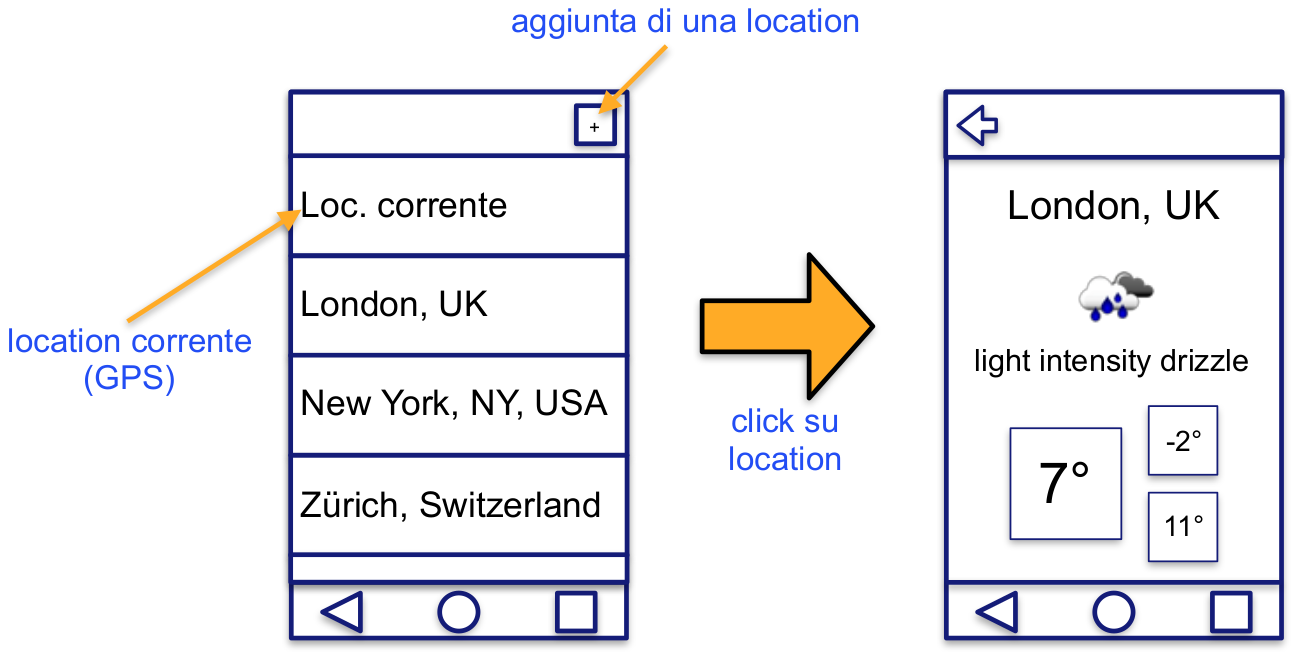
\includegraphics[scale=0.25]{images/fig3.png}
\end{figure}
\section{Requisiti}
\begin{itemize}
    \item Applicazione di tipo List - Detail (vedi Mockup)
    \item Possibilità di aggiungere nuove location manualmente (con popup, nuova
schermata, ...)
    \item Utilizzo del GPS per leggere la posizione corrente e mostrarla in lista
    \item Salvataggio delle location inserite dall'utente su database SQLite
    \item Controllo periodico (tramite Background Service) delle temperature; invio di
notifiche se la temperatura locale scende / sale sopra una certa soglia
\end{itemize}
\section{Features implementate}
\subsection{Current Position}
\subsubsection{Smart Location Library}
Attraverso questa libreria è possibile determinare la posizione geografica del dispositivo utilizzato. Per utilizzarla è necessario aggiungere la
dependecy seguente, all'interno del build.gradle (Module:app):
\begin{lstlisting}
    implementation 'io.nlopez.smartlocation:library:3.3.3'
\end{lstlisting}
Inoltre è necessario inserire nell' AndroidManifest un permesso per identificare la posizione del dispositivo:
\begin{lstlisting}
    <uses-permission android:name="android.permission.ACCESS_COARSE_LOCATION"/>
\end{lstlisting}
Questo permesso è necessario ma non sufficente, dobbiamo richiedere a Runtime, all'utente, un ulteriore permesso
per la localizzazione. Le procedure attorno a cui ruota il meccanismo di richiesta dei permessi
e di localizzazione del device sono:
\begin{lstlisting}
@Override
public void onRequestPermissionsResult(int requestCode,
        @NonNull String[] permissions, @NonNull int[] grantResults) {
    switch (requestCode) {
        case 0: {
            if (grantResults.length > 0 && grantResults[0] 
                            == PackageManager.PERMISSION_GRANTED) {
                Log.d("tag", "Permission granted");
            }
            return;
        }
    }
}

public void startLocationListener() {
    LocationParams.Builder builder = new LocationParams.Builder()
    .setAccuracy(LocationAccuracy.HIGH).setDistance(0)
    .setInterval(500); // mezzo sec
    SmartLocation.with(getActivity()).location().continuous().config(builder.build())
    .start(new OnLocationUpdatedListener() {
        @Override
        public void onLocationUpdated(android.location.Location location) {

            HttpRequestTask requestTask = new HttpRequestTask(ListFragment.this);
            requestTask.execute(
            "https://api.openweathermap.org/data/2.5/weather?lat="
            +location.getLatitude()+"&lon="+location.getLongitude()+
            "&units=metric&appid=ed2aa55e4a426aba9a830d295e909a1a");
        }
    });
}
\end{lstlisting}
\subsubsection{OpenWeatherMap}
Abbiamo utilizzato la smart location library per identificare la posizione del nostro dispositivo.
Grazie alle coordinate geografiche ottenute, eseguiamo una richiesta alle API
OpenWeatherMap, per ottenere il nome e le previsioni meteo della posizione corrente.
La richiesta HTTP è delegata alla classe HttpRequestTask, che estende un task asincrono, in grado
di effettuare richieste HTTP che non influiscano sulla velocità dell'interfaccia grafica.
La risposta HTTP è una stringa Json, per questo motivo è stata sviluppata una classe
OpenWeatherData che funge da container per i dati parsati. Il parsing avviene attraverso
una libreria chiamata Moshi, considerata come un GSON 2.0 scritto in kotlin.
Dopo aver interpretato la risposta il modello viene aggiornato e la modifica viene notificata all'adapter.
Per utilizzare Moshi è necessario aggiungere la seguente dipendenza:
\begin{lstlisting}
    implementation 'com.squareup.moshi:moshi-kotlin:1.8.0'
\end{lstlisting}
Mentre per permettere le richieste HTTP è necessario indicare nel Manifest la seguente permission:
\begin{lstlisting}
    <uses-permission android:name="android.permission.INTERNET" />
\end{lstlisting}
\subsection{Add New Location}
Questa feature è stata implementata utilizzando la classe NewLocationFragment, che estende un 
DialogFragment. Dal ListFragment sull'evento di click del bottone (+) viene eseguito il codice seguente:
\begin{lstlisting}
FragmentManager manager = getFragmentManager();
NewLocationFragment newLocationFragment = new NewLocationFragment();
newLocationFragment.setTargetFragment(ListFragment.this,0);
newLocationFragment.show(manager,"fragment_new_location");
\end{lstlisting}
Il parametro inserito nella form di dialog viene estrapolato attraverso il metodo
onActivityResult. Il dato invece dall'interno del DialogFragment viene esposto con il metodo sendResultBack:
\begin{lstlisting}
public class NewLocationFragment extends DialogFragment{

    EditText input;

    @Override
    public Dialog onCreateDialog(Bundle savedInstanceState) {
        View view = LayoutInflater.from(getActivity())
            .inflate(R.layout.fragment_new_location, null);
        input = view.findViewById(R.id.editText);

        return new AlertDialog.Builder(getActivity())
                .setView(view)
                .setTitle("Add new Location")
                .setPositiveButton(android.R.string.ok, 
                    new DialogInterface.OnClickListener() {
                    @Override
                    public void onClick(DialogInterface dialog, int which) {
                        sendResultBack(Activity.RESULT_OK, 
                                        input.getText().toString());
                    }
                })
                .setNegativeButton(android.R.string.cancel, null)
                .create();
    }

    private void sendResultBack(int resultCode, String name){
        if(getTargetFragment() == null)
            return;
        Intent intent = new Intent();
        intent.putExtra("name", name);
        getTargetFragment().onActivityResult(getTargetRequestCode(),
                                                    resultCode,intent);
    }
}
\end{lstlisting}
\subsection{Data persistence}
Per permettere all'utente di ritrovare le proprie locazioni, dopo un riavvio dell'applicazione, è necessario implementare tecniche per la persistenza dei dati.
Abbiamo utilizzato il database MySqlLite, attraverso le seguenti classi:
\begin{itemize}
    \item \textbf{DatabaseHelper}\\ Questa classe, estendendo SQLiteOpenHelper, si occupa della creazione delle tabelle a seguito del primo avvio dell'applicazione.
    \begin{lstlisting}
        @Override
        public void onCreate(SQLiteDatabase db) {
            db.execSQL("create table " + DbSchema.LocationsTable.NAME + "("
                            + " _id integer primary key autoincrement, "
                            + DbSchema.LocationsTable.Cols.UUID
                            + ", "
                            + DbSchema.LocationsTable.Cols.NAME
                            + ")"
            );
        }
    \end{lstlisting}
    \item \textbf{DbSchema}\\ Questa classe statica definisce lo schema del Database, è utilizzata per evitare che i nomi delle tabelle e dei
    loro attributi vengano harcodati.
    \item \textbf{LocationsCursorWrapper}\\ Questa classe è il cursore che ci permette di accedere in lettura ai dati, estende CursorWrapper, e definisce
    al suo interno dei metodi che ci facilitino nelle operazioni di lettura dei contenuti.
\end{itemize}
\subsection{ViewPager}
Il ViewPager permette all’utente di navigare attraverso delle view facendo lo ”swipe” con il dito (a de-
stra o a sinistra). Per utilizzarlo è stato necessario definirlo all'interno di un layout
e definire i metodi di supporto richiesti da tale oggetto, all'interno della classe DetailActivity:
\begin{lstlisting}
    @Override
    protected void onCreate(Bundle savedInstanceState) {
        super.onCreate(savedInstanceState);
        setContentView(R.layout.detail_pager);
        UUID entryId = (UUID) getIntent().getSerializableExtra(EXTRA_LOCATION_ID);
        mViewPager = findViewById(R.id.entry_view_pager);
        mEntries = LocationsHolder.get(this).getLocations();
        FragmentManager fragmentManager = getSupportFragmentManager();
        mViewPager.setAdapter(new FragmentStatePagerAdapter(fragmentManager) {
            @Override
            public Fragment getItem(int position) {
                Location entry = mEntries.get(position);
                return DetailLocationFragment.newInstance(entry.getId());
            }
            @Override
            public int getCount() {
                return mEntries.size();
            }});
        for (int i = 0; i < mEntries.size(); i++) {
            if (mEntries.get(i).getId().equals(entryId)) {
                mViewPager.setCurrentItem(i);
                break;
    }    }}
\end{lstlisting}
\subsection{Graphic User Interface}
L'interfaccia grafica utilizza delle risorse drawable che, prima di essere state aggiunte ai file di progetto, sono state processate da un tool online, per la
creazione dei file multimediali con le differenti risoluzioni.
L'applicazione è in grado di cambiare lo sfondo della pagina di dettaglio e la relativa icona, in base alle condizioni climatiche della location interessata. E' stato definito un layout di dettaglio apposito, per la modalità landscape.
\subsection{Temperature Monitoring Service}
Questa classe si occupa di eseguire il check periodico della temperatura nella location corrente e di inviare una notifica in caso in cui la temperatura superi o si abbassi oltre i valori di soglia predefiniti.
Per eseguire questo check periodicamente, anche quando l'applicazione non è in esecuzione, utilizziamo un servizio di sistema chiamato AlarmManager, che permette di inviare degli intent.
La nostra classe TemperatureMonitoringService, che estende IntentService, ricevendo questo intent, si attiverà. L'AlarmManager viene informato sul tipo di Intent da inviare attraverso la classe PendingIntent.
Attraverso il metodo onHandleIntent possiamo definire il comportamento del service, alla ricezione di un Intent:
\begin{lstlisting}
@Override
protected void onHandleIntent(Intent intent) {
    Log.i(TAG, "Received an intent: " + intent);
    if (ContextCompat.checkSelfPermission(this,
    Manifest.permission.ACCESS_FINE_LOCATION)== PackageManager.PERMISSION_GRANTED) {
        LocationParams.Builder builder = new LocationParams.Builder().
                setAccuracy(LocationAccuracy.HIGH).setDistance(0)
                .setInterval(500); // mezzo sec
        SmartLocation.with(this).location().continuous()
        .config(builder.build()).start(new OnLocationUpdatedListener() {
            @Override
            public void onLocationUpdated(android.location.Location location) {

                HttpRequestTask requestTask = 
                    new HttpRequestTask(TemperatureMonitoringService.this);
                requestTask.execute(
                    "https://api.openweathermap.org/data/2.5/weather?lat="
                    +location.getLatitude()+"&lon="+location.getLongitude()
                    +"&units=metric&appid=ed2aa55e4a426aba9a830d295e909a1a");
            }
        });
}}
\end{lstlisting}
\vspace{0,3cm}
Quando il Task richiamato dal service terminerà la sua esecuzione, verrà invocato il metodo seguente,
che eseguirà il parsing della stringa Json ritornata ed eventualmente inviarà una notifica:\\
\begin{lstlisting}
@Override
public void onHttpRequestTaskCompleted(String result) throws IOException {
    Moshi moshi = new Moshi.Builder().build();
    JsonAdapter<OpenWeatherData> jsonAdapter = moshi.adapter(OpenWeatherData.class);
    OpenWeatherData openWeatherData = jsonAdapter.fromJson(result);
    if(openWeatherData.getTemperature().getTemp() >= HOT_THRESHOULD){
        sendNotification("Attention, today it is very hot, remember to drink a lot!");
        Log.d(TAG,"sendNotification1");
    }else if(openWeatherData.getTemperature().getTemp() <= COLD_THRESHOULD){
        sendNotification("Attention, today it is very cold, the road can be icy!");
        Log.d(TAG,"sendNotification2");
}   }
\end{lstlisting}
\section{Risultati ottenuti}
\begin{figure}[!htb]
    \minipage{0.23\textwidth}
      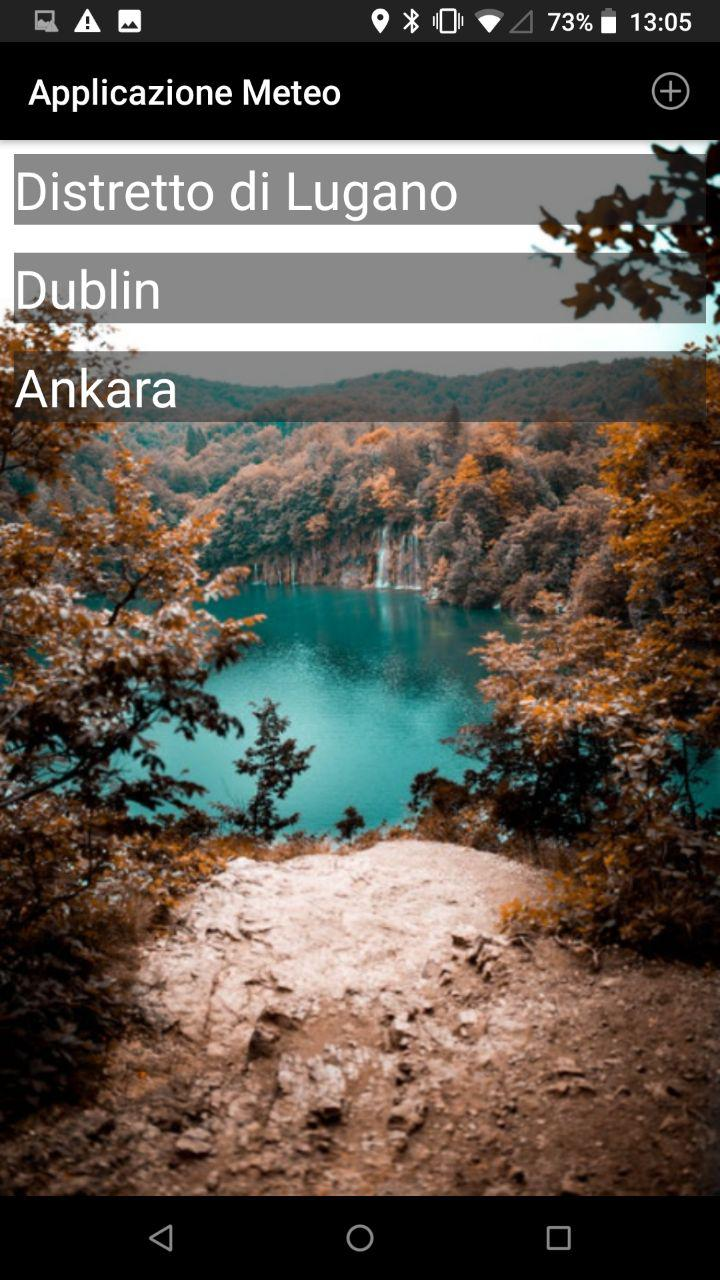
\includegraphics[width=\linewidth]{images/sc2.jpg}
      \caption{Main view}\label{fig:awesome_image1}
    \endminipage\hfill
    \minipage{0.23\textwidth}
      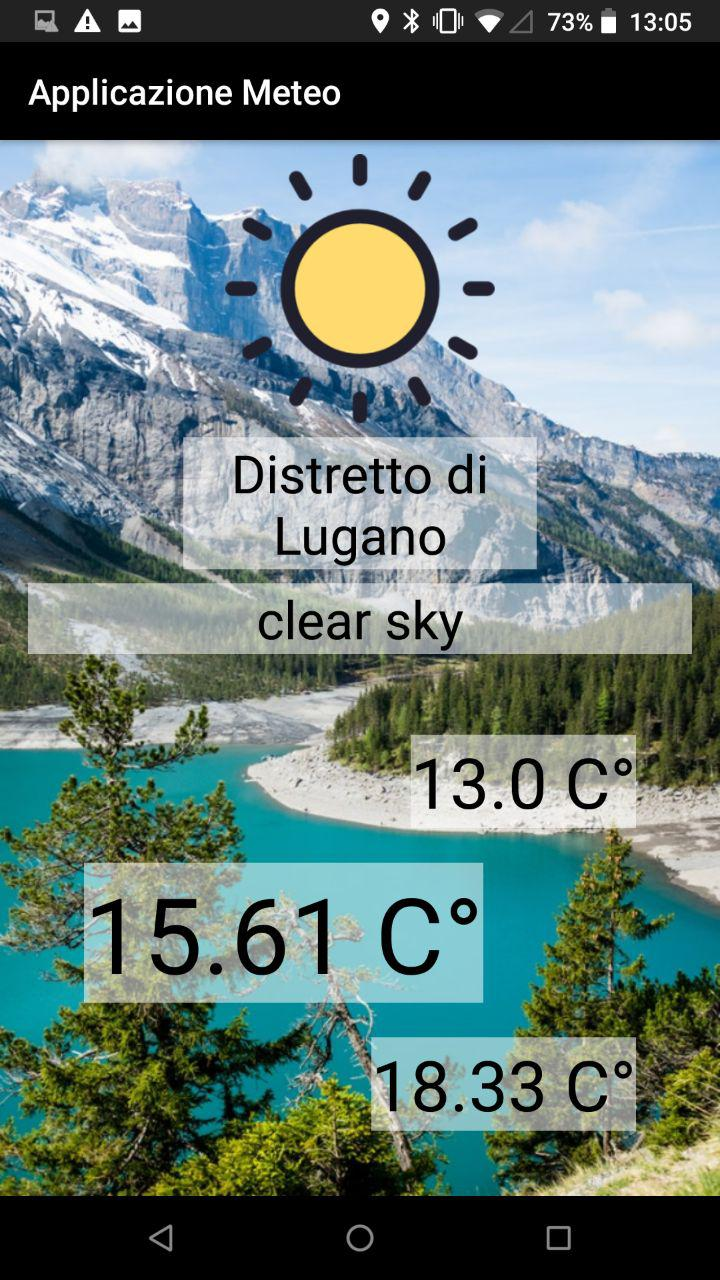
\includegraphics[width=\linewidth]{images/sc3.jpg}
      \caption{Detail view}\label{fig:awesome_image2}
    \endminipage\hfill
    \minipage{0.23\textwidth}%
      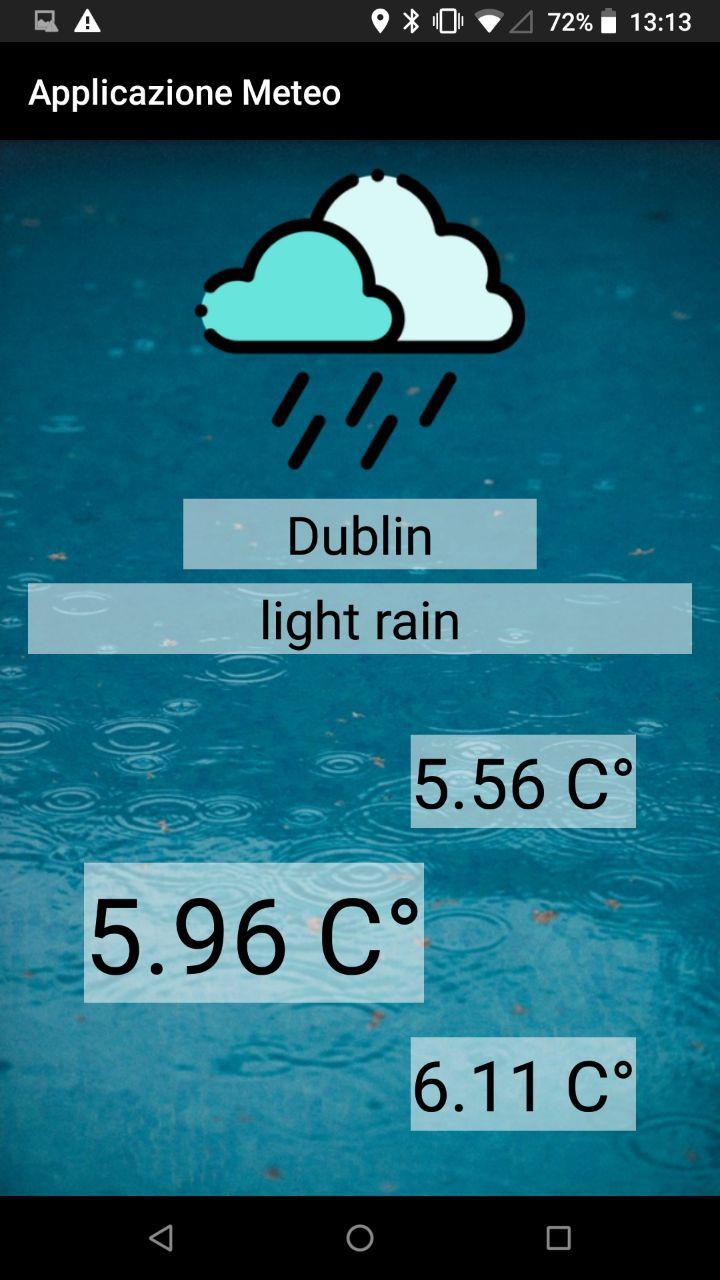
\includegraphics[width=\linewidth]{images/sc4.jpg}
      \caption{Detail view}\label{fig:awesome_image3}
    \endminipage\hfill
    \minipage{0.23\textwidth}%
      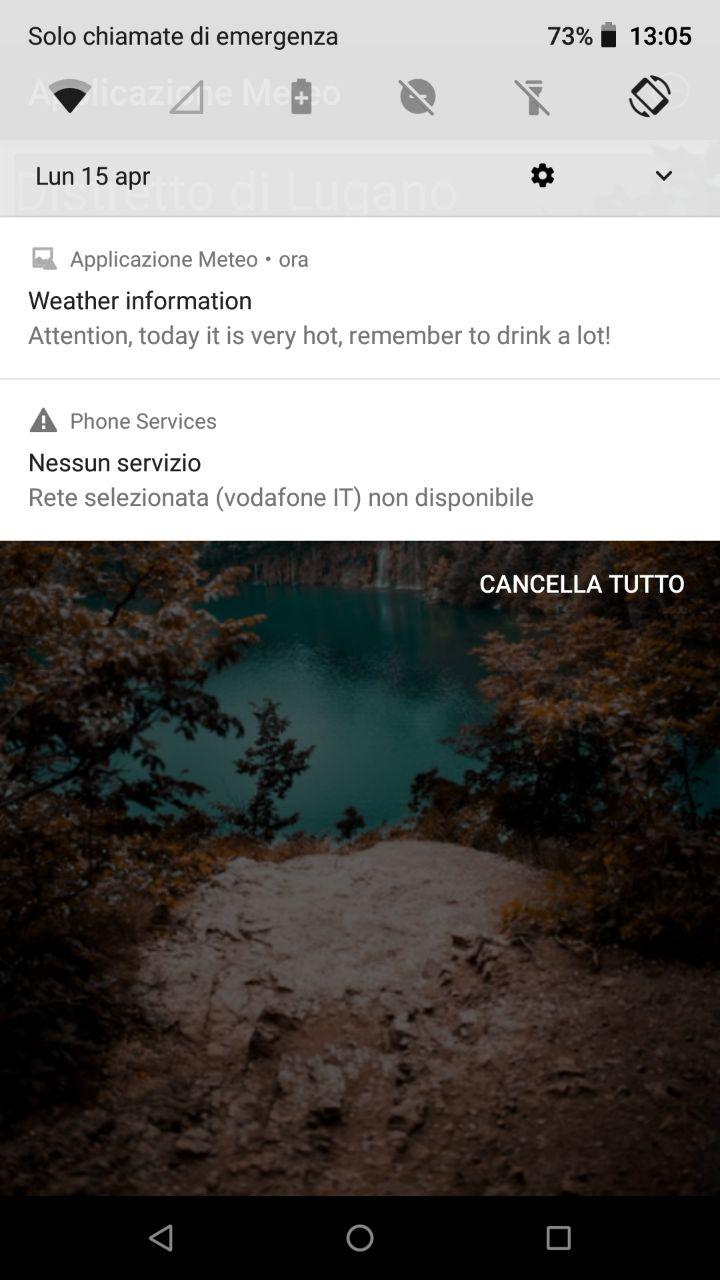
\includegraphics[width=\linewidth]{images/sc1.jpg}
      \caption{Notification}\label{fig:awesome_image3}
    \endminipage
\end{figure}
\noindent Nelle immagini sopra riportate si osservano le viste principali dell'applicazione:
\begin{itemize}
    \item \textbf{Figure 1:} Vista principale dell'applicazione, in questa sezione è possibile inserire una nuova località e visualizzarla a schermo, insieme alla località corrente.
    \item \textbf{Figure 2-3:} Cliccando su una località all'interno della lista è possibile visualizzarne la pagina di dettaglio in cui vengono riportati i dati relativi al nome della località, alla descrizione delle condizioni atmosferiche e alla temperatura massima, minima e corrente.
    \item \textbf{Figure 4:} Periodicamente viene inviata una notifica nel caso in cui la temperatura corrente superi o si abbassi entro alcune soglie. I contenuti del messaggio possono essere i seguenti: \\\\ \textit{"Attention, today it is very hot, remember to drink a lot!"} \\ \textit{"Attention, today it is very cold, the road can be icy!"}
\end{itemize}
\end{document}